\subsection{Energispektrum}
\label{sec:energispektrum}

% \begin{figure}[h!]
%   \centering
%   \subbottom[Dobbeltkoincidenser]{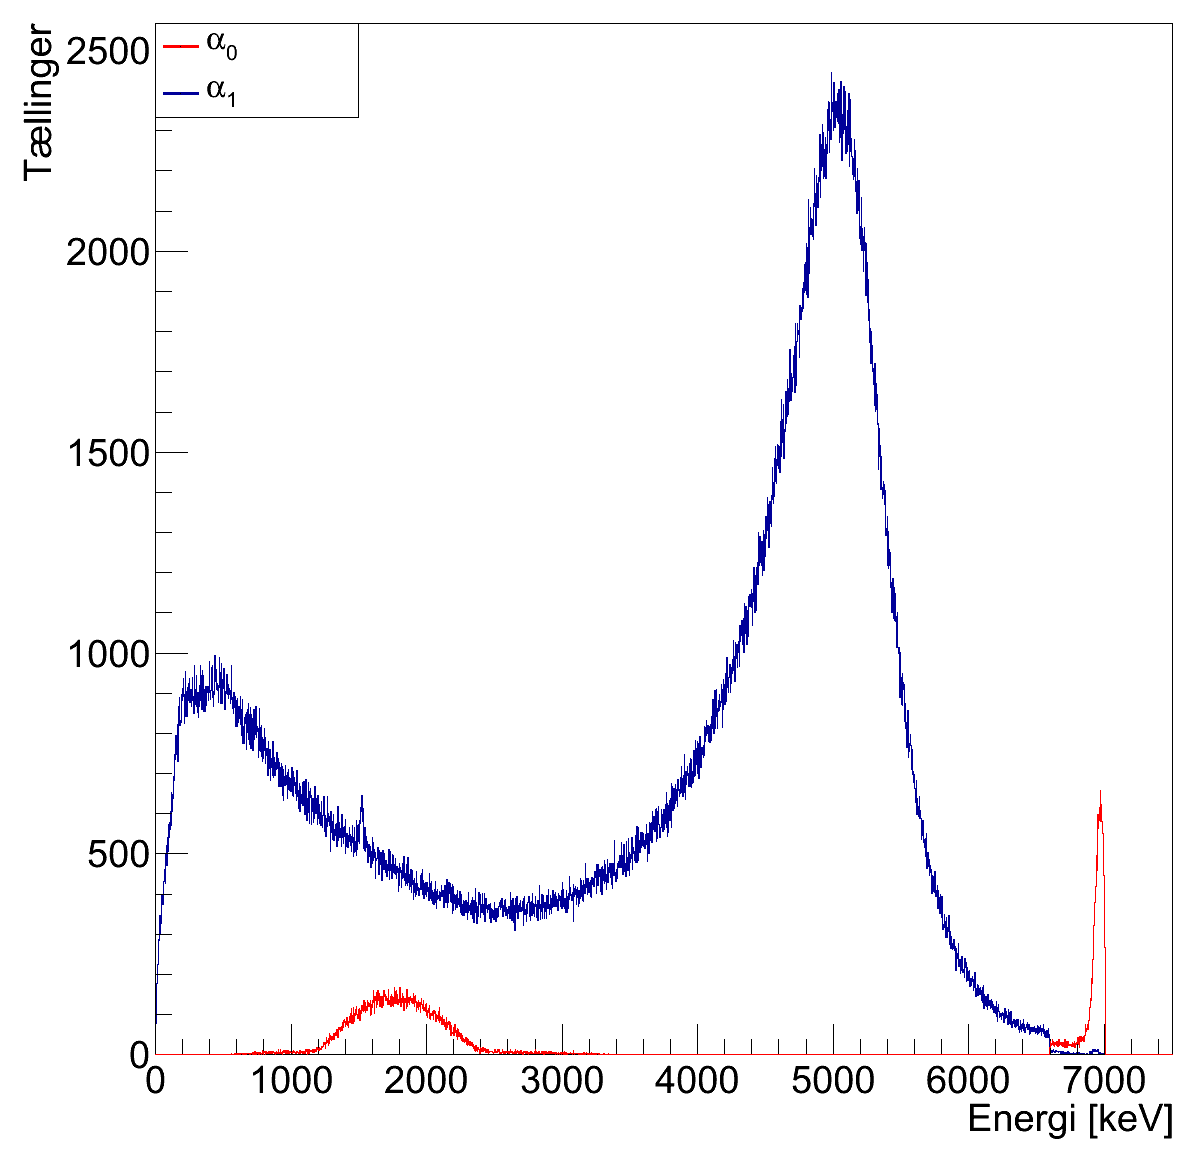
\includegraphics[width=0.47\columnwidth]{1077-spec-D-mix}}%
%   \hfill
%   \subbottom[Trippelkoincidenser]{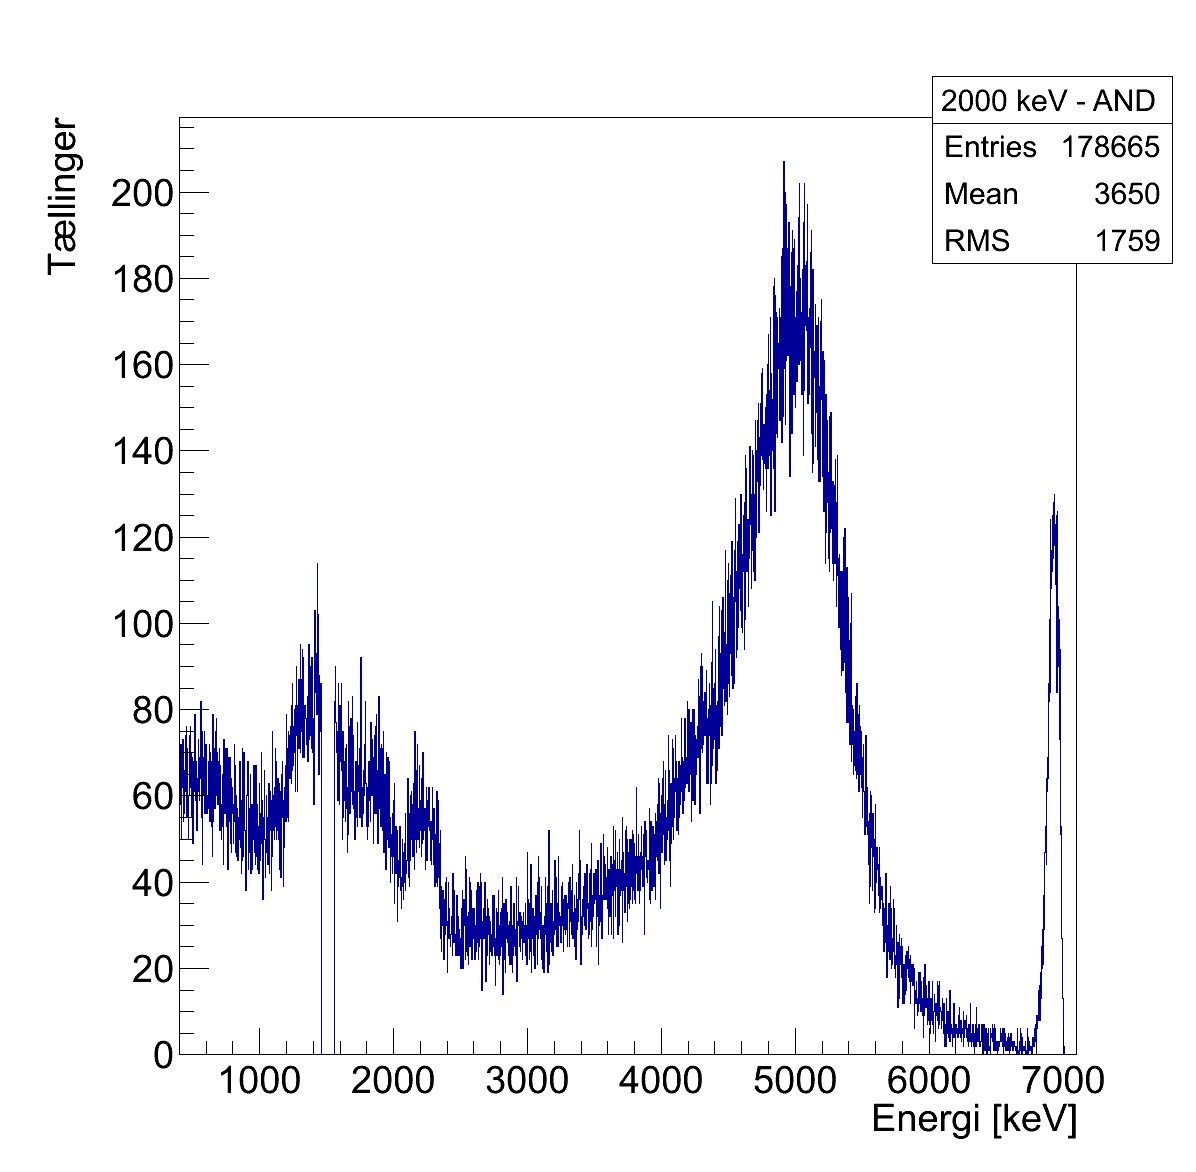
\includegraphics[width=0.47\columnwidth]{1077-spec-T}}%
%   \caption{Antal tællinger som funktion af energien for henfald fra \SI{17.8}{\MeV}. Den smalle
%     $\alpha_{0}$ og den brede $\alpha_{1}$ top ses tydeligt.}
%   \label{fig:alphaSpectrum}
% \end{figure}

\begin{figure}[h!]
  \centering
  \vspace{-0.3cm}
  \subbottom[Dobbeltkoincidenser - \SI{17.8}{\MeV}]{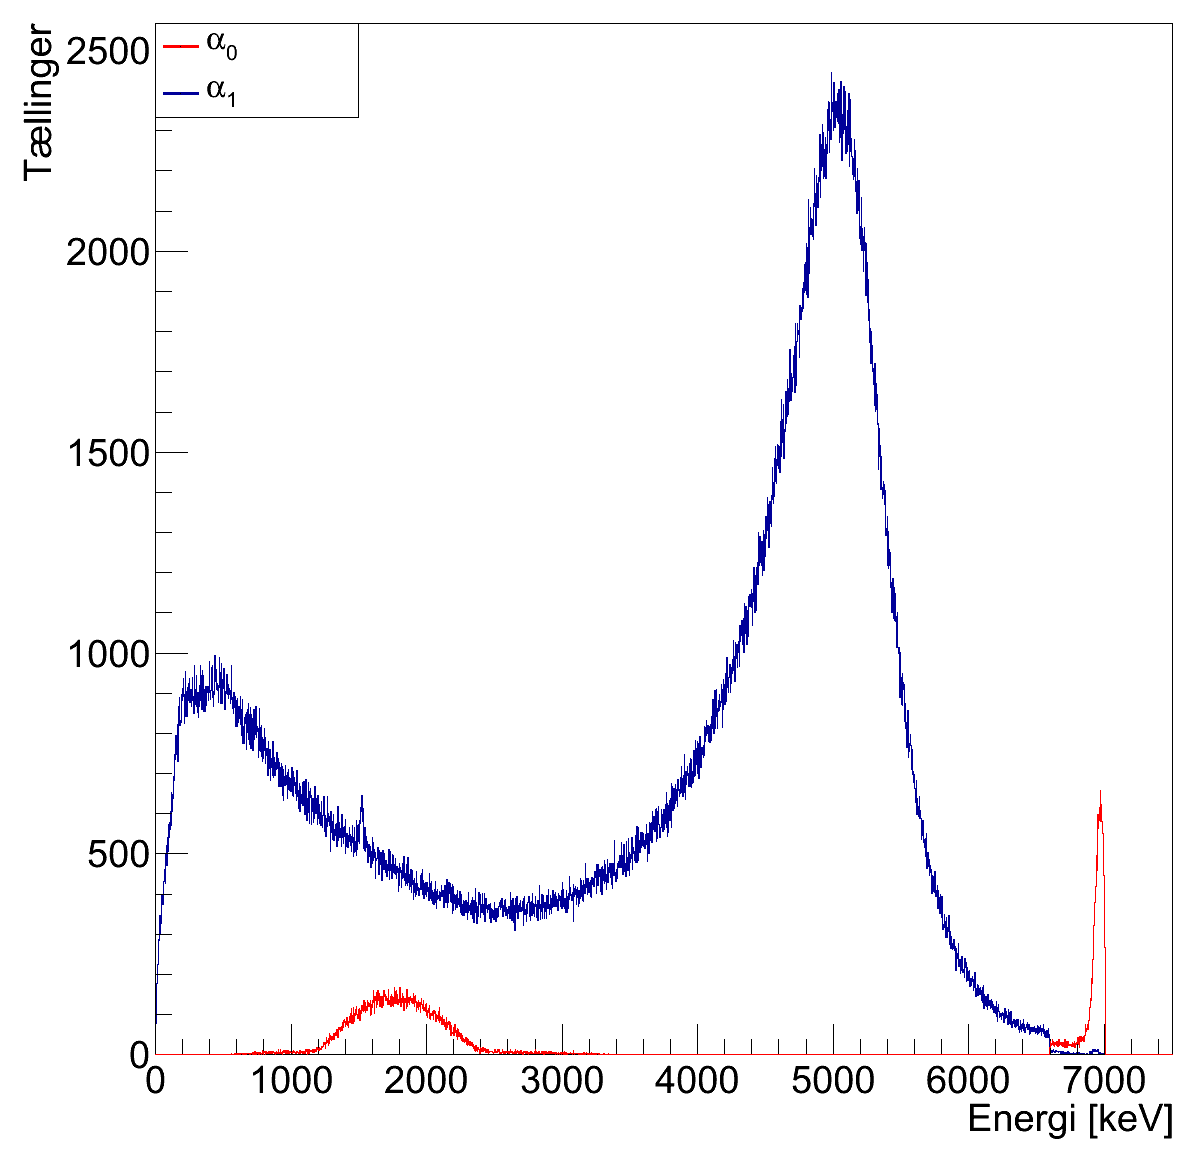
\includegraphics[width=0.45\columnwidth]{1077-spec-D-mix}}%
  \hfill
  \subbottom[Trippelkoincidenser-
  \SI{17.8}{\MeV}]{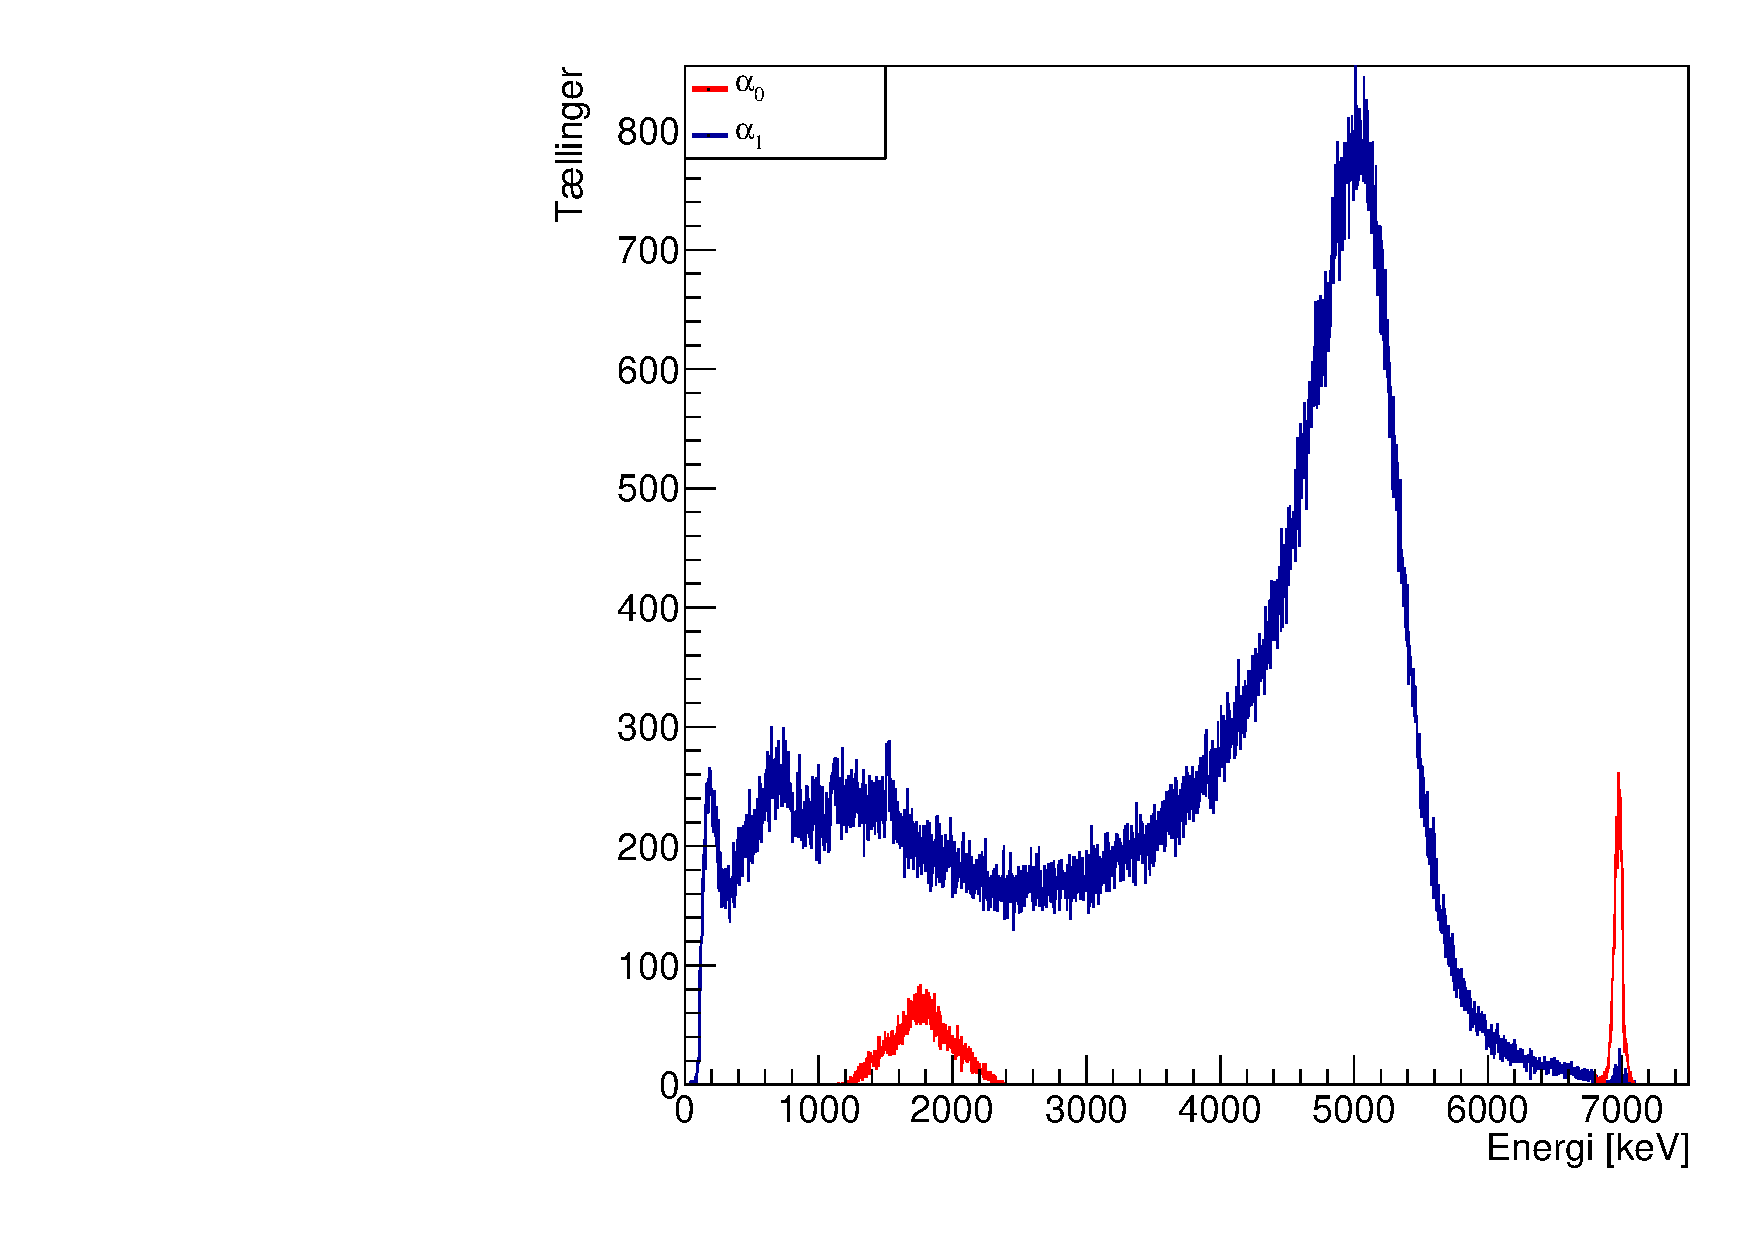
\includegraphics[width=0.45\columnwidth]{1077-spec-T-mix}}%
  \\
%  \caption{Antal tællinger som funktion af energien for \SI{17.8}{\MeV} tilstanden.}
%  \label{fig:alpha-1077}
  %
  %
  %
  \subbottom[Dobbeltkoincidenser - \SI{18.2}{\MeV}]{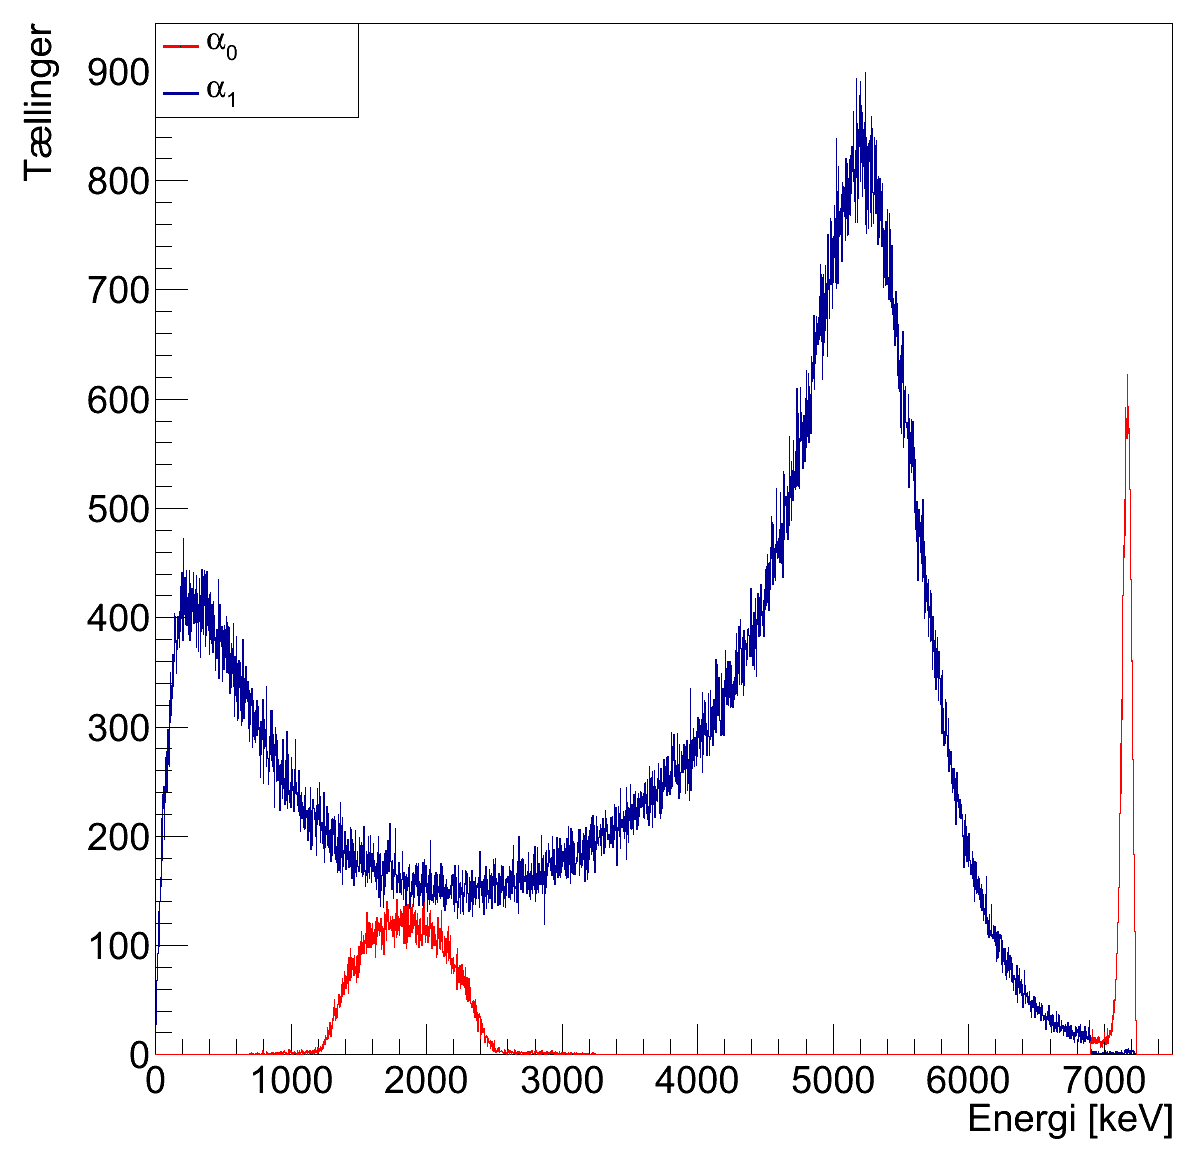
\includegraphics[width=0.45\columnwidth]{1108-spec-D-mix}}%
  \hfill
  \subbottom[Trippelkoincidenser - \SI{18.2}{\MeV}]{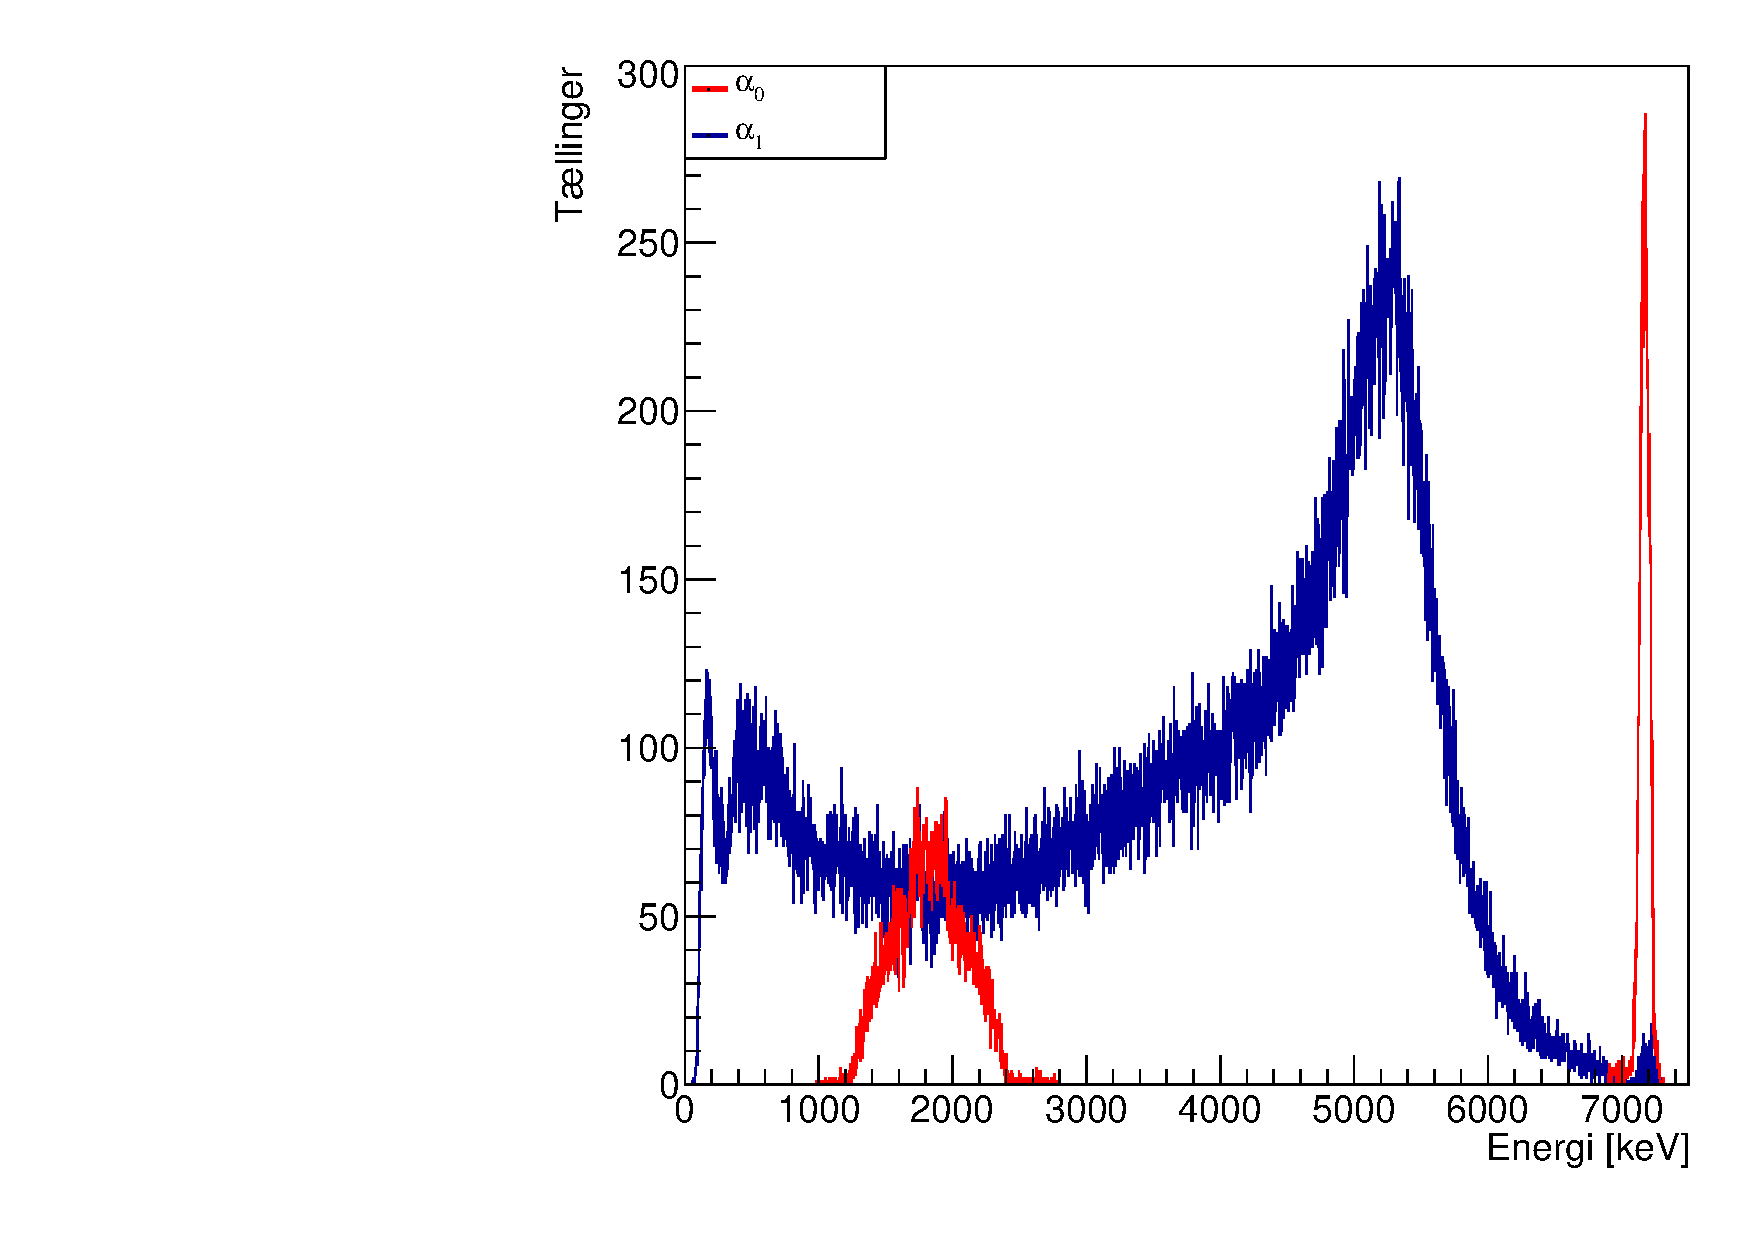
\includegraphics[width=0.45\columnwidth]{1108-spec-T-mix}}%
  \\
  % \caption{Antal tællinger som funktion af energien for \SI{18.2}{\MeV} tilstanden.}
%  \label{fig:alpha-1108}
  %
  %
  %
  \subbottom[Dobbeltkoincidenser - \SI{18.5}{\MeV}]{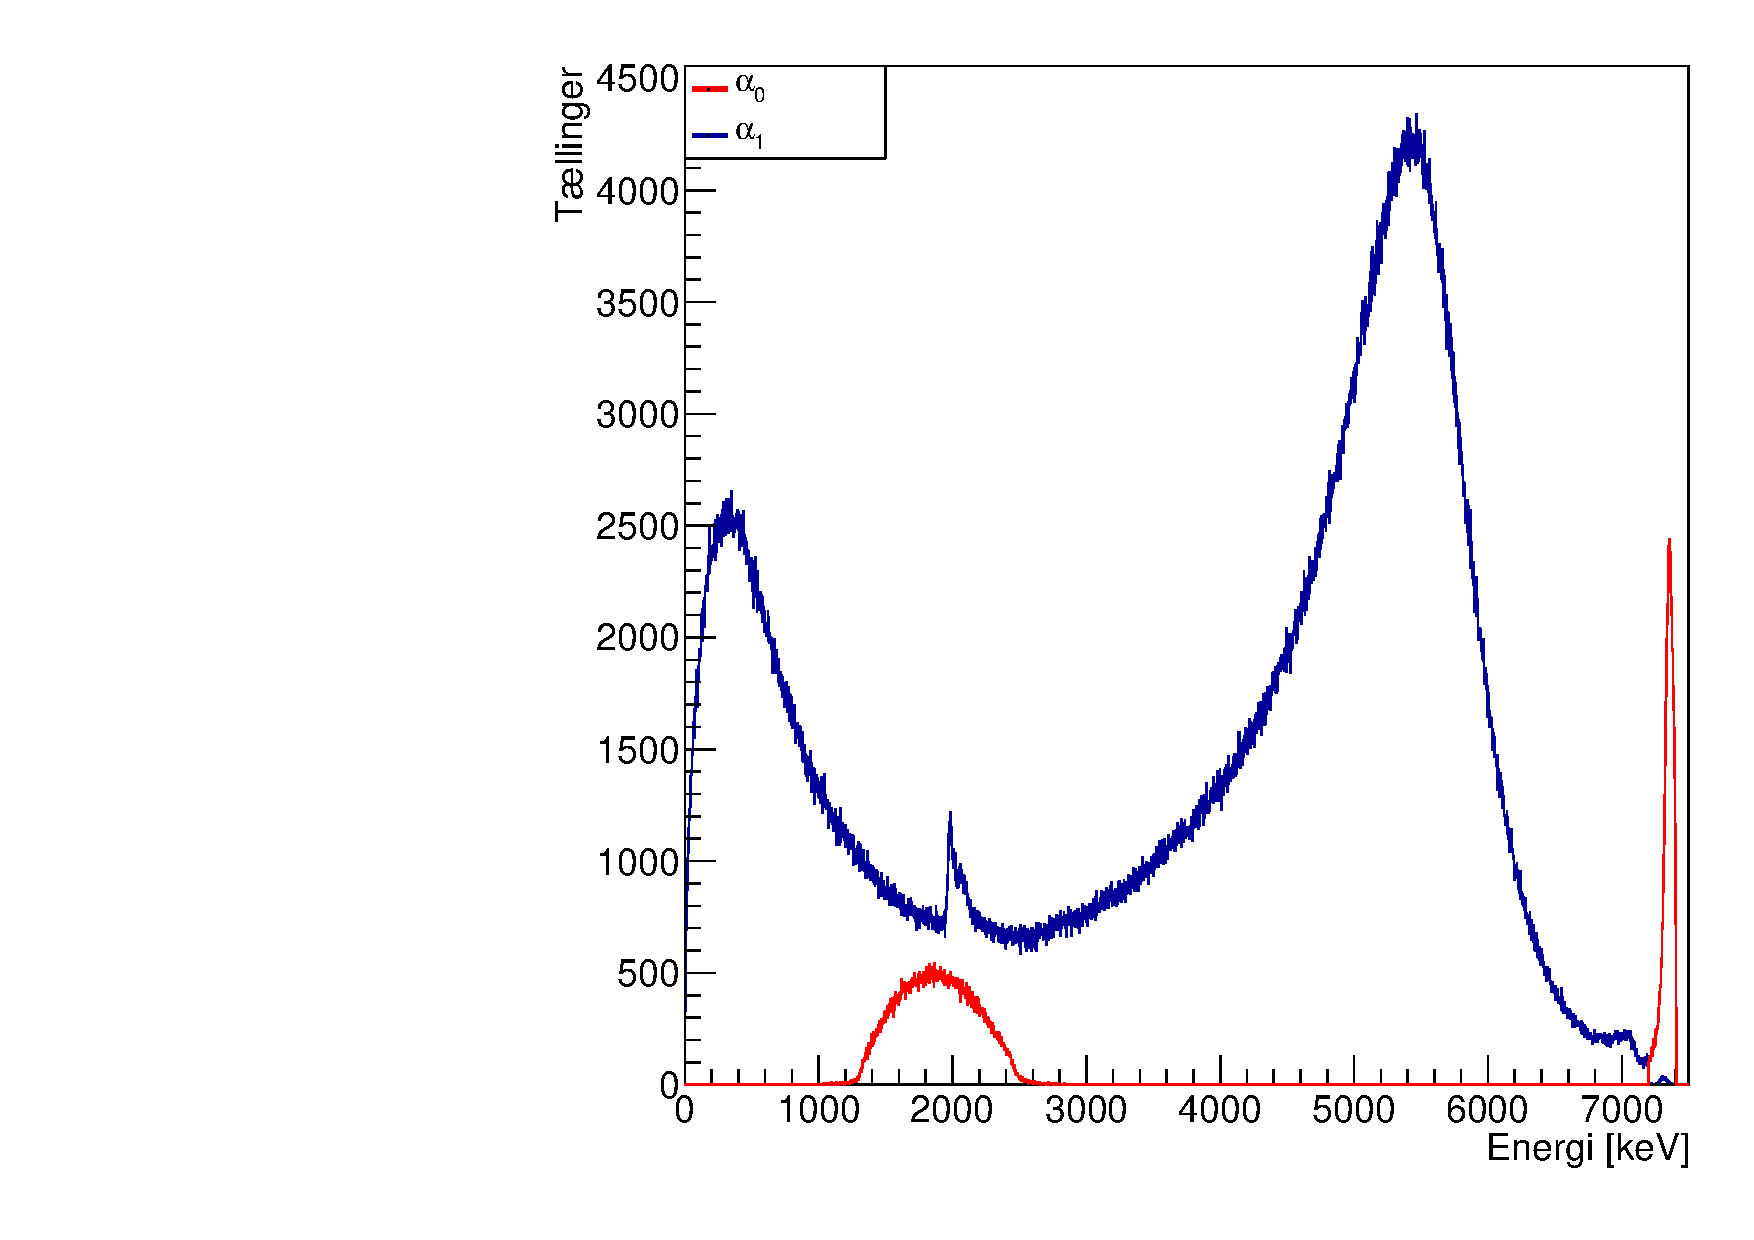
\includegraphics[width=0.45\columnwidth]{1128-spec-D-mix}}%
  \hfill
  \subbottom[Trippelkoincidenser - \SI{18.5}{\MeV}]{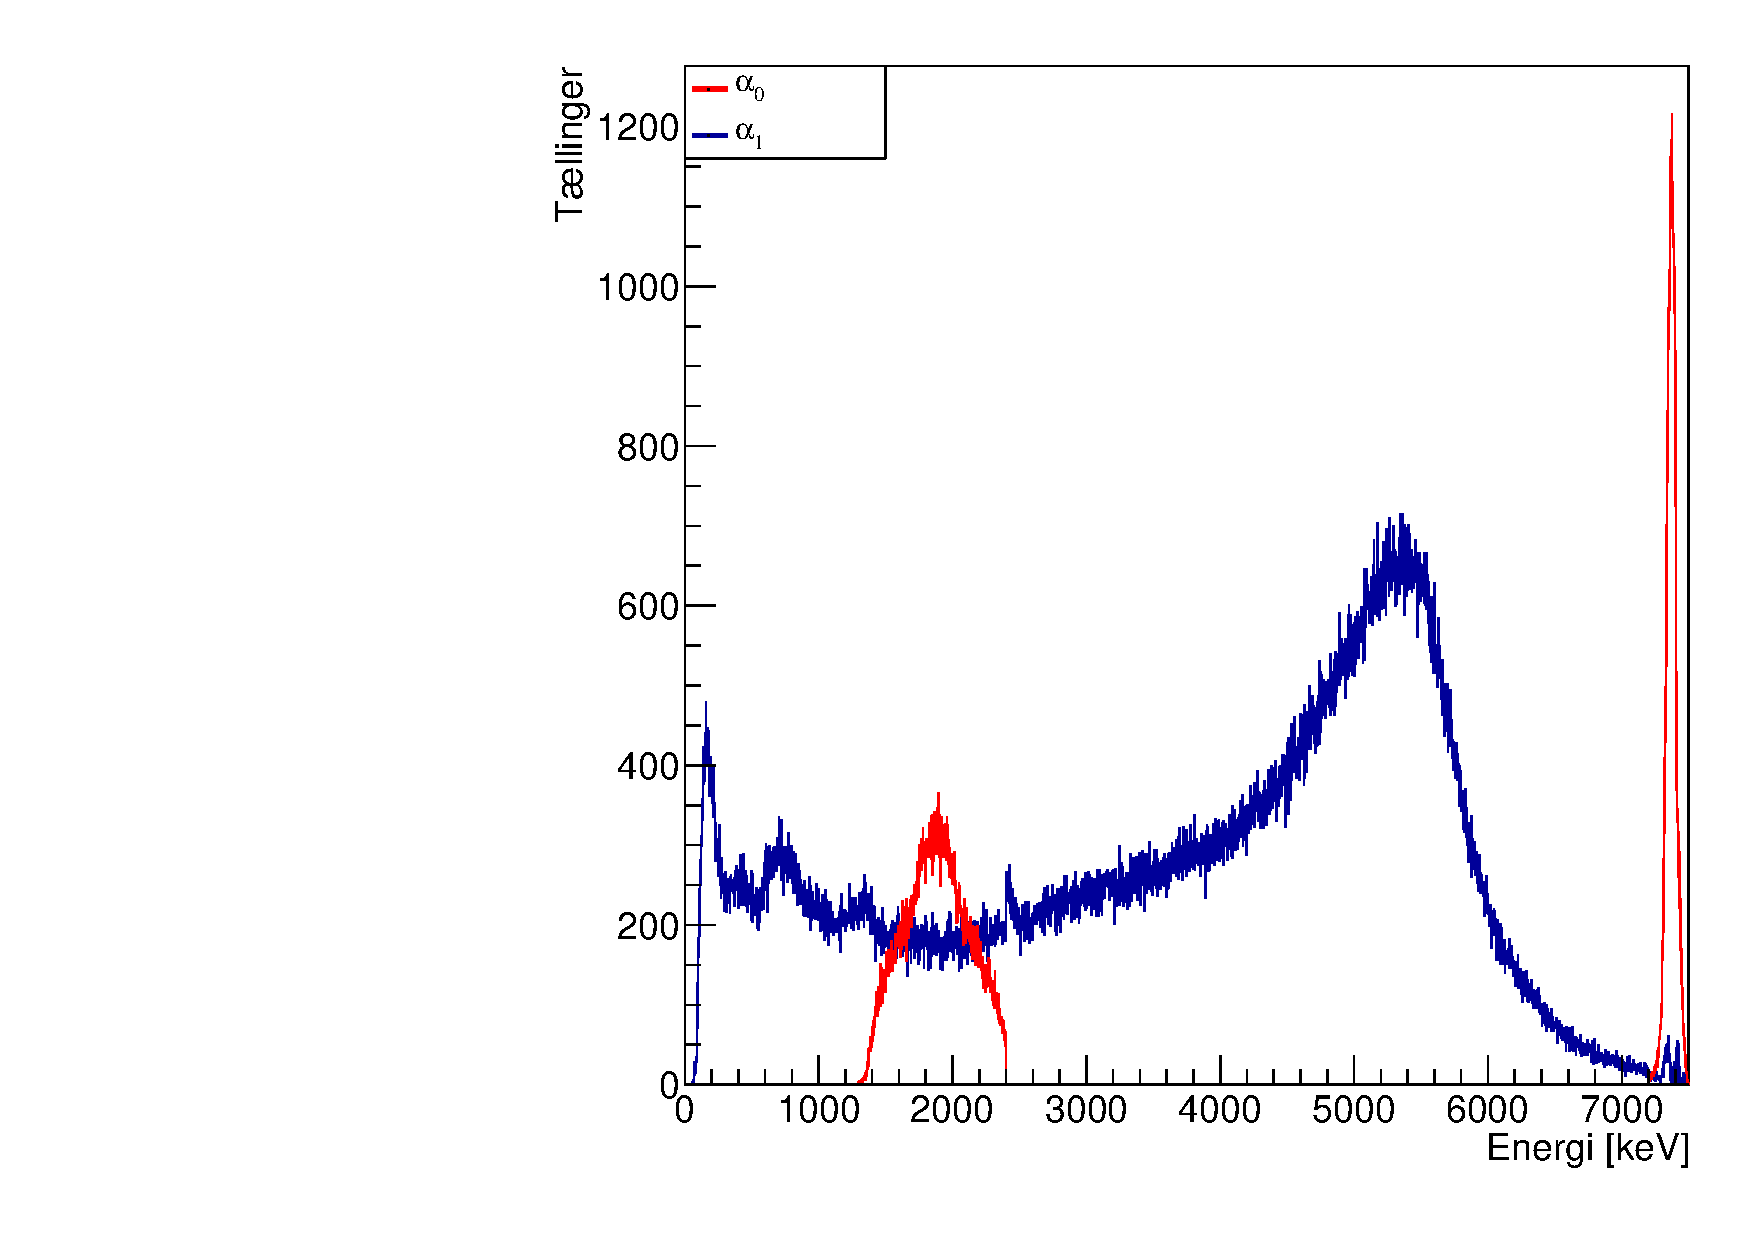
\includegraphics[width=0.45\columnwidth]{1128-spec-T-mix}}%
  \caption{Antal tællinger som funktion af energien i CM. \Carb excitationsenergien er angivet under de
    enkelte figurer. Den røde kurve angiver spektret for $\alpha_{0}$ og dennes sekundære partikler. Den
    blå kurve er det tilsvarende for $\alpha_{1}$.}
  \label{fig:alpha-spec}
  \vspace{-1.3cm}
\end{figure}

På \cref{fig:alpha-spec} ses $\alpha$-spektret i CM for henfald til grundtilstanden og første exciterede
tilstand for hhv. dobbelt- og trippelkoincidenser, hvor der er benyttet 2, \num{2.37} og
\SI{2.65}{\MeV} protoner. Ifølge \cite{States} populerer dette hhv.  en $0^{+}$ isospin 1 tilstand i
\Carb med excitationsenergi \SI{17.8}{\MeV}, en $1^{+}$ isospin 0 tilstand ved \SI{18.2}{\MeV} og en
$3^{-}$ isospin 1 ved \SI{18.5}{\MeV}.

% For dobbeltkoincidenserne består den blå kurve kun de hændelser, hvor en af partiklerne ikke er en
% $\alpha_{0}$ svarende til $\alpha_{1}$ spektret. Den røde kurve er så fundet ved at trække den blå fra det
% samlede spektrum for dermed at opnå $\alpha_{0}$ spektret. Tilsvarende er den røde kurve for
% trippelkoincidenserne de hændelser hvor der ikke var nogen $\alpha_{1}$. Den blå kurve angiver her det
% samlede spektrum 

I alle spektre ses tydeligt en smal top omkring 7\MeV. Under denne ligger en bred Breit-Wigner
lignende top centreret omkring 5\MeV. Disse toppe stemmer fint overens med, hvad det forventes for
$\alpha_{0}$ og $\alpha_{1}$ i forhold til, hvad der forventes for bredde og energi.
$\alpha_{1}$-toppen er dog ikke perfekt Breit-Wigner fordelt, hvilket skyldes, at
tunneleringssandsynligheden afhænger kraftigt af energien. Endvidere er der også et lille bidrag til
asymmetrien fra de sekundære partikler. Desuden ses det, at fordelingen af de sekundære partikler
fra $\alpha_{0}$-henfald har samme form i alle tre trippelkoincidensspektre. Tilsvarende gør sig gældende
for de sekundære partikler fra $\alpha_{1}$ i dobbeltkoincidensspektrene.

Figurerne viser også både styrken og svagheden ved dobbeltkoincidenserne. De bidrager med meget
data, men samtidig er der også større chance for støj fra protonstrålen, som det tydeligt ses på
\cref{fig:alpha-spec}e og mindre tydeligt på \cref{fig:alpha-spec}a. Støjen er her placeret ved
samme energi som \cref{eq:rutherUdCM} forudsiger.

De målte spektre er dermed i overensstemmelse med hypotesen om sekventielt henfald til tre
$\alpha$-partikler via \Be. Endvidere må det konkluderes, at alle tre tilstande indeholder en isospin 0
komponent, da henfald via tre $\alpha$-partikler ellers ikke ville være muligt. 

De to midterste paneler på \cref{fig:alpha-spec} viser spektret fra en tilstand med unaturlig paritet. I
\cref{sec:pop-beryllium} blev det udledt, at en tilstand med unaturlig paritet ikke kan henfalde til
grundtilstanden af \Be. Ifølge \cite{States} har tilstanden isospin 0 og $\alpha$-henfald fra denne vil
derfor være mere hyppige end fra de omkringliggende isospin 1 tilstande. Dette er dog langt fra
tilfældet, idet $\alpha_{0}$-henfald udgør en væsentlig andel både af dobbelt- og
trippelkoincidensspektret. Data er dermed ikke i overensstemmelse med en $1^{+}$ isospin 1 tilstand
ved \SI{18.2}{\MeV} i \Carb, hvilket stemmer fint overens med, at \cite{States} ikke er sikre på
deres konklusion.


\subsubsection{Eksperimentelle detektoreffekter}
\label{sec:data-detek}

Forholdet mellem de to toppe i dobbeltkoincidensspektrene stemmer fint overens med det forventede med
en kraftig undertrykkelse af $\alpha_{0}$-toppen.

For trippelkoincidenserne forventes flest $\alpha_{0}$, hvis tværsnittet af $\alpha_{0}$ og
$\alpha_{1}$ er den samme.

For spektret på \cref{fig:alpha-spec}b er det modsatte tilfældet. Forklaringen kan være, at
tværsnittet for $\alpha_{1}$ er væsentligt større. Dette virker umiddelbart modstridende, idet
tunneleringssandsynligheden for $\alpha$-henfald afhænger kraftigt af
energien. Tunneleringssandsynligheden er nært relateret til levetiden og et udtrykt er udledt i
\cite[s. 236]{Martin}
\begin{equation}
  \label{eq:SStunnel}
  \lambda \propto w(\alpha) e^{-G}, \qquad G \propto \frac{Z}{\sqrt{E_{\alpha}}}.
\end{equation}
Umiddelbart taler ovenstående også for henfald med $\alpha_{0}$, men faktoren $w(\alpha)$ skal dog
bemærkes. Denne er en "fittefaktor"{} for at få teorien til at passe med de eksperimentelle
data. Faktoren angiver sandsynlighen for at finde $\alpha$-partiklen inden for kernen. Fortolkningen af
trippelkoincidensspektret er derfor, at det er mere sandsynligt, at $\Carb(\SI{17.8}{\MeV})$ består
\Be i en $2^{+}$ tilstand sammen med en $L=2$ $\alpha$-partikel, end $0^{+}$ \Be sammen med
en $L=0$ $\alpha$-partikel. Dette stemmer overens med de tabulerede værdier af tværsnittet i
\cite{States}, der angiver værdierne $\sigma(\alpha_{0}) = \SI{9}{\mb}$ og
$\sigma(\alpha_{1}) = \SI{25}{\mb}$. Værdien for tværsnittet af $\alpha_{1}$-processen er dog mere usikker.

Tværsnittene for \SI{18.5}{\MeV} tilstanden er hhv.  $\sigma(\alpha_{0}) = \SI{32.4\pm4.8}{\mb}$ og
$\sigma(\alpha_{1}) = \SI{270\pm40}{\mb}$, men på trods af det, dominerer $\alpha_{1}$-toppen ikke dennes
trippelkoincidensspektrum. Forholdet mellem tværsnittene stemmer dog ikke overens med de oplyste
bredder i samme tabel, som er hhv.  $\Gamma_{\alpha_{0}} = \SI{65}{\keV}$ og
$\Gamma_{\alpha_{1}} = \SI{177}{\keV}$. På baggrund af dette er konklusionen, at de opnåede data ikke er
konstistente med de oplyste tværsnit i \cite{States}, men at denne tabel heller ikke er
selvkonsistent.

Ser man på fordelingen af de sekundære partikler fra $\alpha_{0}$-henfaldet, fremgår det tydeligt, at
fordelingen har én form i alle dobbeltkoincidensspektrene og en anden i
trippelkoincidensspektret. Desuden kan fordelingen af de sekundære partikler fra $\alpha_{1}$ i
dobbeltkoincidenserne nemt identificeres, hvor den i trippelkoincidenserne primært ligner støj.

På baggrund af dette afsnit kan det konkluderes, at den præcise modulering af spektret er meget
afhængig af koincidensbetingelserne, samt den specifikke opstilling. For de undersøgte tilstande er
de dog nogenlunde ens. For at opnå fuld forståelse af fordelingen er det
derfor nødvendigt at foretage en simulering. Dette ligger dog uden for tidsrammen af dette
projekt. Dobbelt- og trippelkoincidenserne vil derfor behandles separat i den videre analyse.
